\chapter{Network Layer\label{chap:networklayer}}
\todo{Ausarbeitung von Felix Graf durchlesen, versch Georouting erkl�ren, bilder einf�gen. Auf Problemstellung eingehen}
\section{Congestion Control\label{sec:congestioncontrol}}
\section{Geo Routing\label{sec:georouting}}
Da sich die Fahrzeuge andauernd mit hoher Geschwindigkeit bewegen und sich dadurch die Topologie des Netzes st�ndig �ndert, sind verschiedene Addressierungsmethoden definiert. Diese sind als ETSI-Standart aufgef�hrt und umfasse die Folgenden Szenarien. 

\begin{figure}
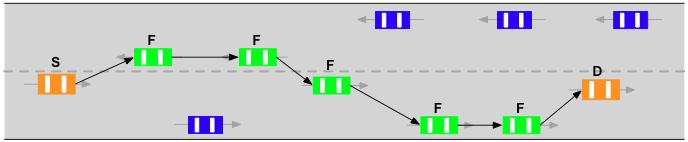
\includegraphics[width=0.99\textwidth]{content/images/03_networklayer/GeoUnicast.jpg}
\caption{Geo Unicast \cite{etsi102636-1}}
\label{fig:geounicast}
\end{figure}

\begin{figure}
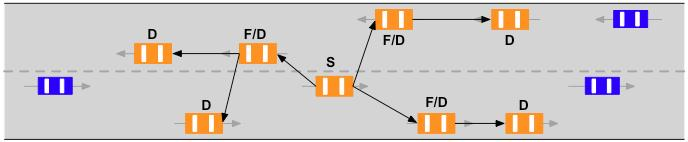
\includegraphics[width=0.99\textwidth]{content/images/03_networklayer/TSC.jpg}
\caption{Topologically-scoped broadcast \cite{etsi102636-1}}
\label{fig:tsc}
\end{figure}

\begin{figure}
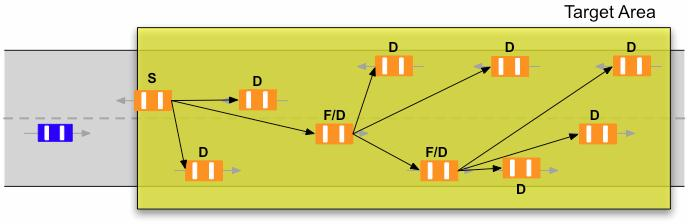
\includegraphics[width=0.99\textwidth]{content/images/03_networklayer/GSB.jpg}
\caption{geographically-scoped broadcast \cite{etsi102636-1}}
\label{fig:gsb}
\end{figure}
